\label{WG3}

\subsection{Large R jets and boosted object tagging in ATLAS -- C. F. Anders}
At the high center of mass energies of the Large Hadron Collider even the heaviest known Standard Model particles can be observed with large transverse momenta, in the so called boosted topology. Boosted $W$ and Higgs bosons and top quarks that decay to quarks will be highly collimated and can therefore be reconstructed in a single jet with large radius parameter $R$. In ATLAS the jets are reconstructed with the anti-k$_t$~\cite{Cacciari:2008gp} algorithm, usually requiring a transverse momentum of $p_T>200$~GeV and a radius parameter of $R=1.0$ and are trimmed~\cite{Krohn:2009th} with the parameters  $R_{\mathrm{sub}}=$ 0.2 and $f_{\mathrm{cut}}=$ 5\%. 

To distinguish signal, e.g.\ real $W$ bosons from QCD induced jet backgrounds one of the main observables is the jet mass, calculated from the jet constituents. In Figure \ref{fig:jetmass_W} the distribution of the jet mass in data and simulation is shown after a lepton + jet selection that aims at selecting $t\bar{t}$ events. It shows a clear peak at the expected Standard Model $W$ boson mass. Using a further discriminating variable $W$ boson taggers are build that have a fixed signal efficiency of 50\% and reduce the background by a factor of 50.
\begin{figure}[!h]
\begin{centering}
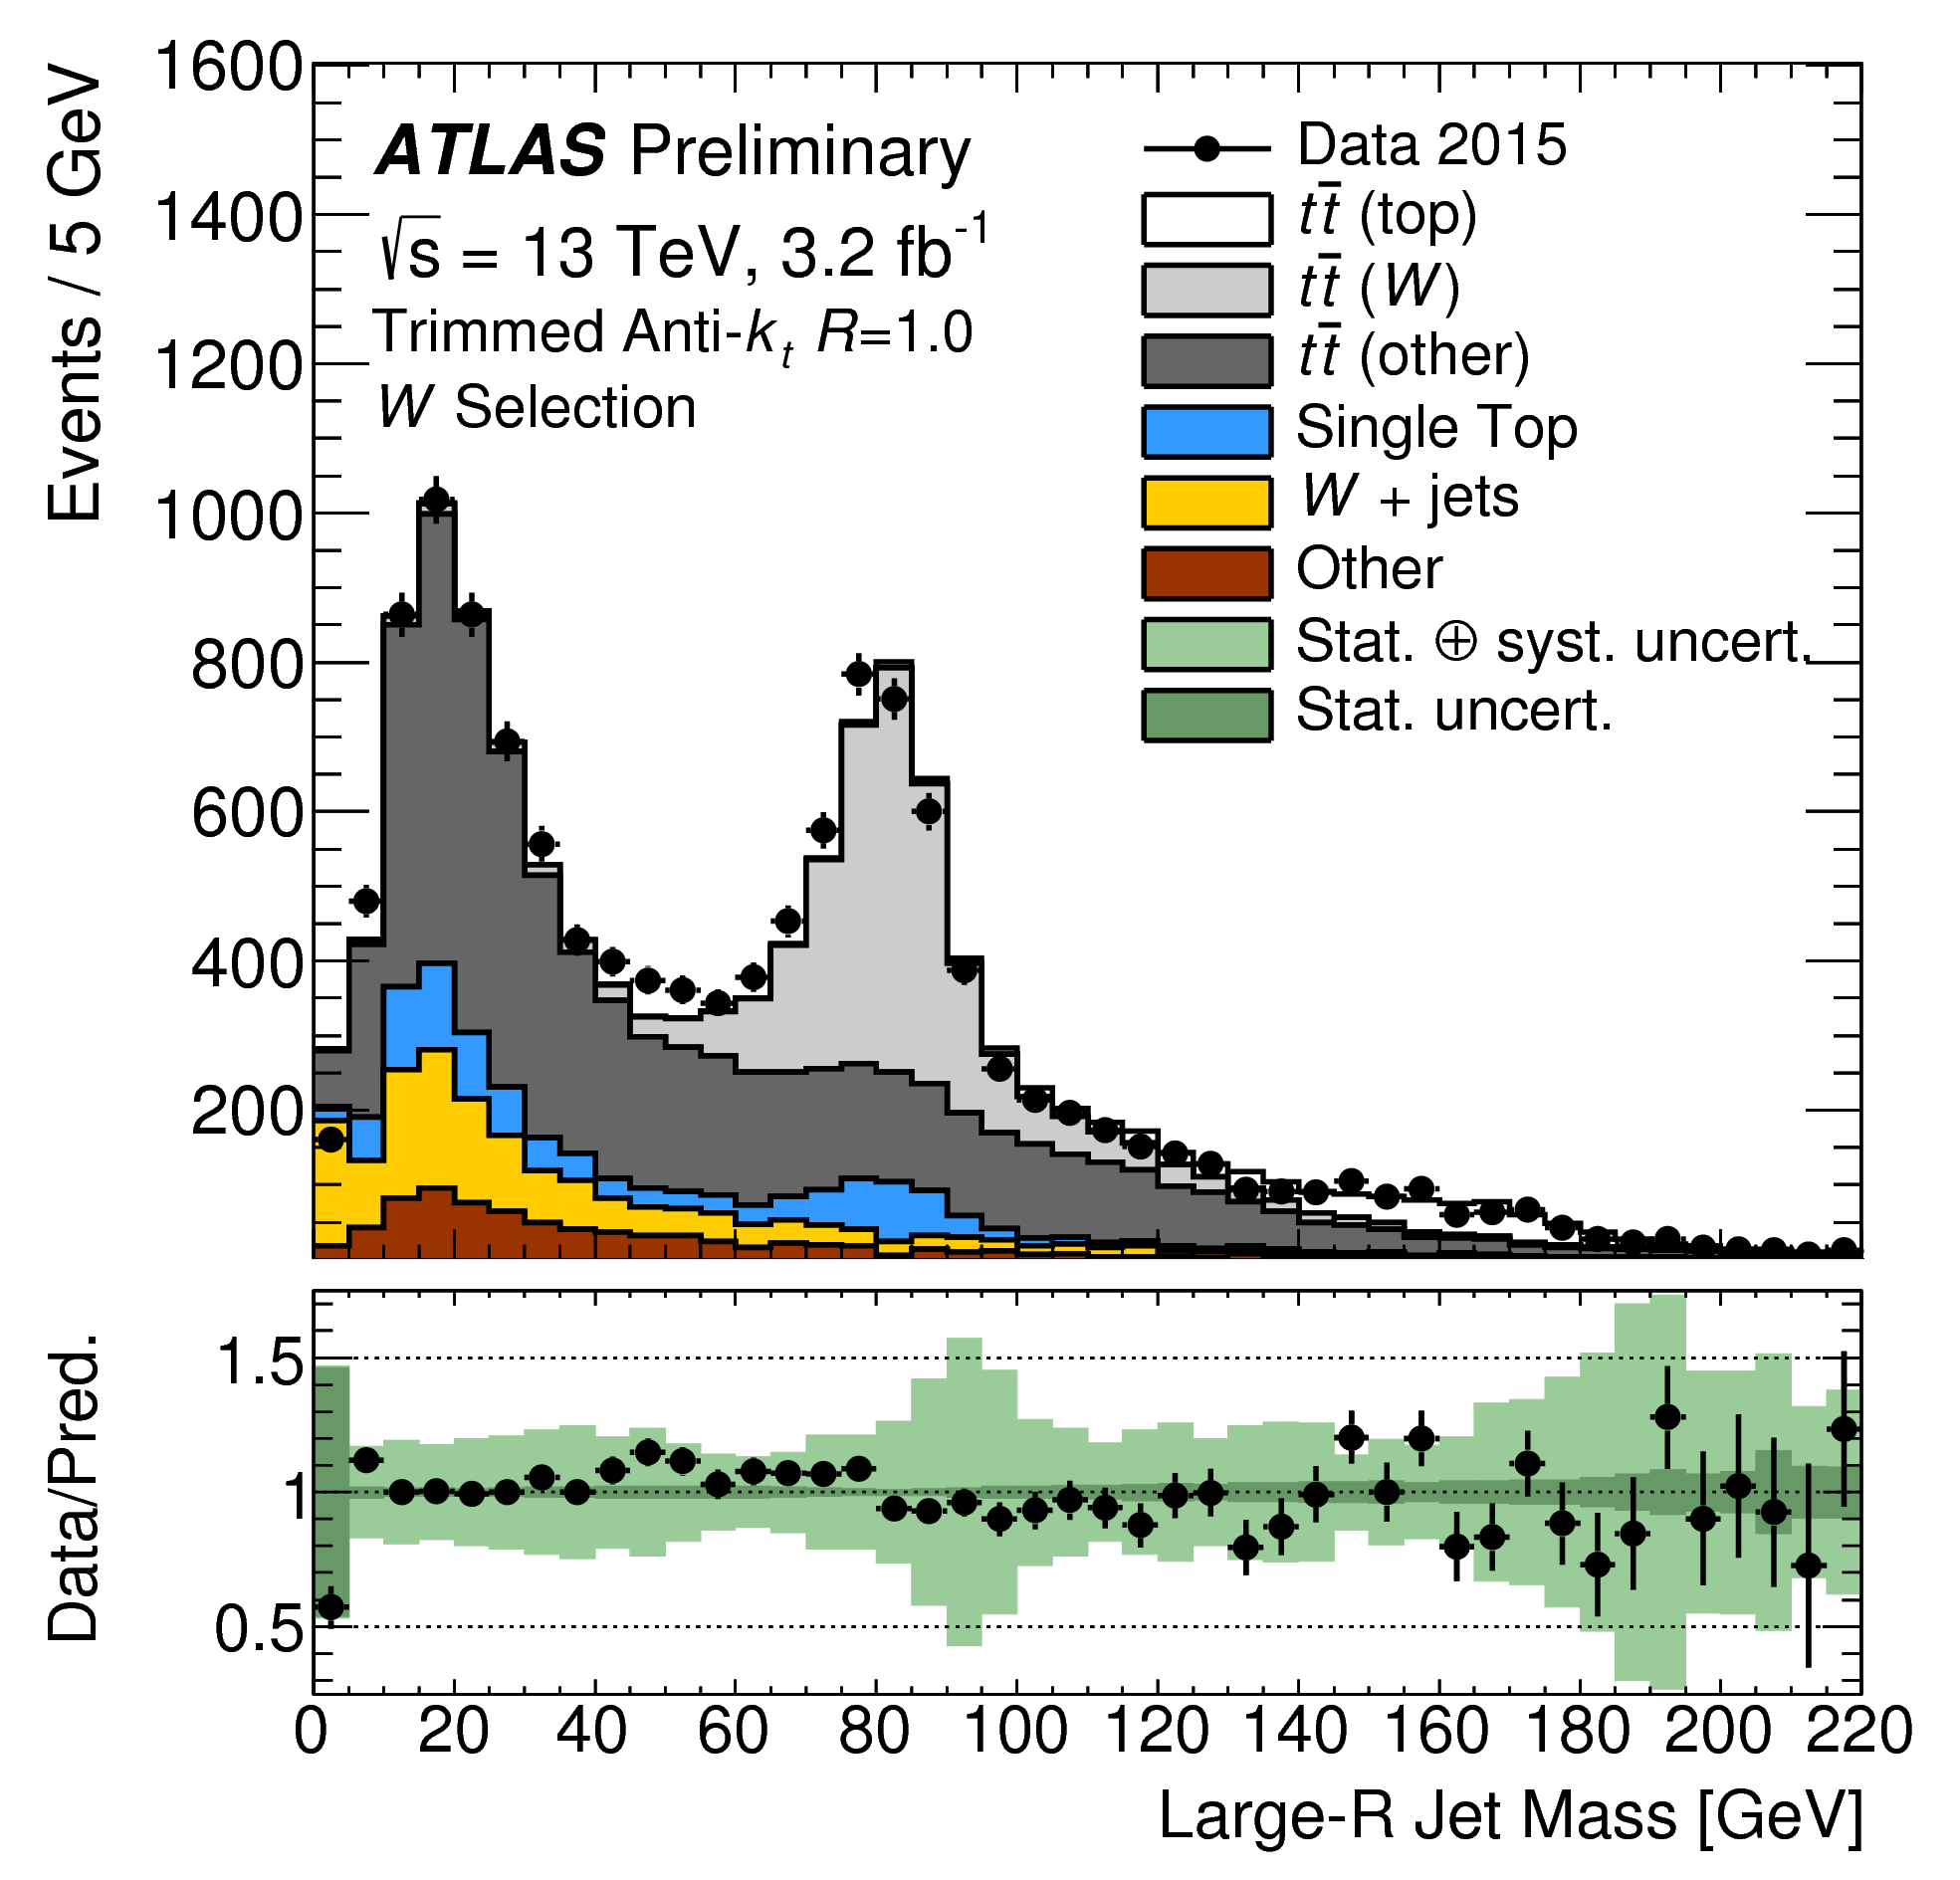
\includegraphics[width=0.48\textwidth]{WG3_plots/fig_07}
\caption{Distribution of the calorimeter jet mass spectrum for the leading-p$_T$ jet in 13 TeV data and MC simulation using trimmed (J. High Energ. Phys. (2010) 2010: 84.) anti-k$_t$ R=1.0 jets  with trimming parameters $f_{\mathrm{cut}}=5$\% and $R_{\mathrm{sub}} = 0.2$ in lepton+jets events. The large $R$ jets are required to have $p_T>200$ GeV. (cite: http://atlas.web.cern.ch/Atlas/GROUPS/PHYSICS/PLOTS/JETM-2016-005/)}
\label{fig:jetmass_W}
\end{centering}
\end{figure}

Recently, the possibilities of adding more information and exploiting multi-dimensional corelations has been explored by using Boosted Descicion Trees (``BDT'') and Deep Neural Networks (``DNN'') to tag boosted hadronically decaying $W$ bosons. Compared to simple 2-variable tagging approaches the multivariate approaches perform better, as can be seen in Figure \ref{fig:MVA}.



\begin{figure}[!h]
\begin{centering}
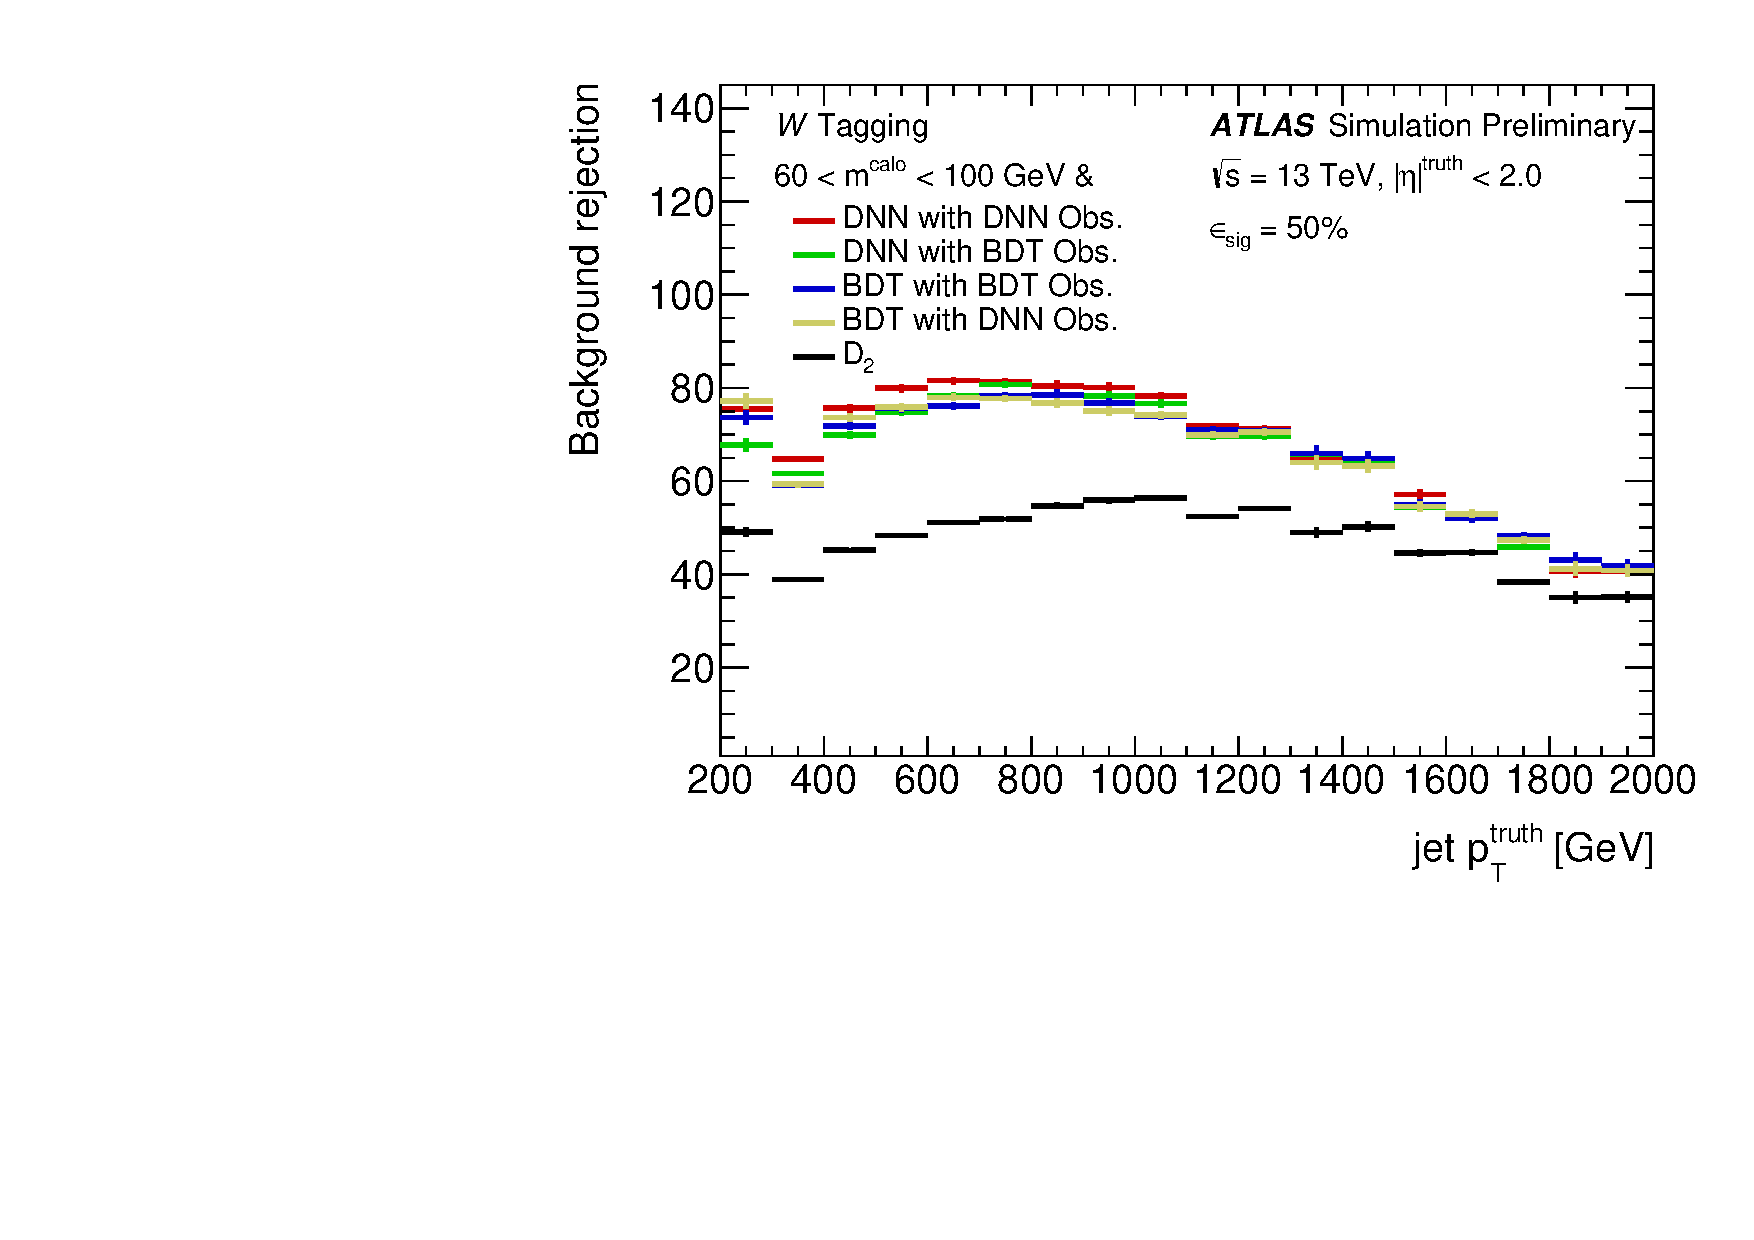
\includegraphics[width=0.48\textwidth]{WG3_plots/fig_07c}
\caption{Distributions showing comparison of the BDT and DNN taggers performance to a simple W tagger. (http://atlas.web.cern.ch/Atlas/GROUPS/PHYSICS/PUBNOTES/ATL-PHYS-PUB-2017-004/)}
\label{fig:MVA}
\end{centering}
\end{figure}



\subsection{Jet substructure techniques for VBS in CMS -  A. Hinzmann}

Jet identification techniques that make use of jet substructure information are important tools for the measurement of VBS.
A brief summary of the existing tools used by the CMS experiment and future prospects for the HL-LHC is given in the following.

To probe high WW, ZZ or WZ invariant masses, special jet identification techniques for W and Z bosons decaying to quarks are needed, since for high momentum W and Z bosons, the shower of hadrons originating from the quark anti-quark pair merges into a single large radius jet of particles~\cite{CMS-PAS-JME-16-003, CMS-PAS-JME-14-002, Khachatryan:2014vla}.
The maximum angular separation between the quark and anti-quark is given by $\Delta R_{q\bar{q}}=2 m / p_{T}$, where $m$ and $p_T$ are the mass and transverse momentum, respectively, of the W or Z boson.
For a W boson with $p_T=1$ TeV, an angular separation of  $\Delta R_{q\bar{q}}=0.2$ is expected, which is well below the typical jet size parameter of 0.4 used by CMS.
At even higher $p_T=3.5$ TeV, the angular distance $\Delta R_{q\bar{q}}=0.05$ between the decay products of a W boson is even smaller than the granularity of the hadron calorimeter of CMS with cell sizes of $\Delta \eta \times \Delta \phi = 0.087 \times 0.087$ in the barrel region of the detector.
CMS thus employs a particle-flow event algorithm~\cite{CMS-PRF-14-001} to measure jet substructure, that reconstructs and identifies each individual particle with an optimized combination of information from the various elements of the CMS detector, benefiting from spatial and energy resolution of all sub-detectors.

\begin{figure}[htb]
% \hspace{-2cm}
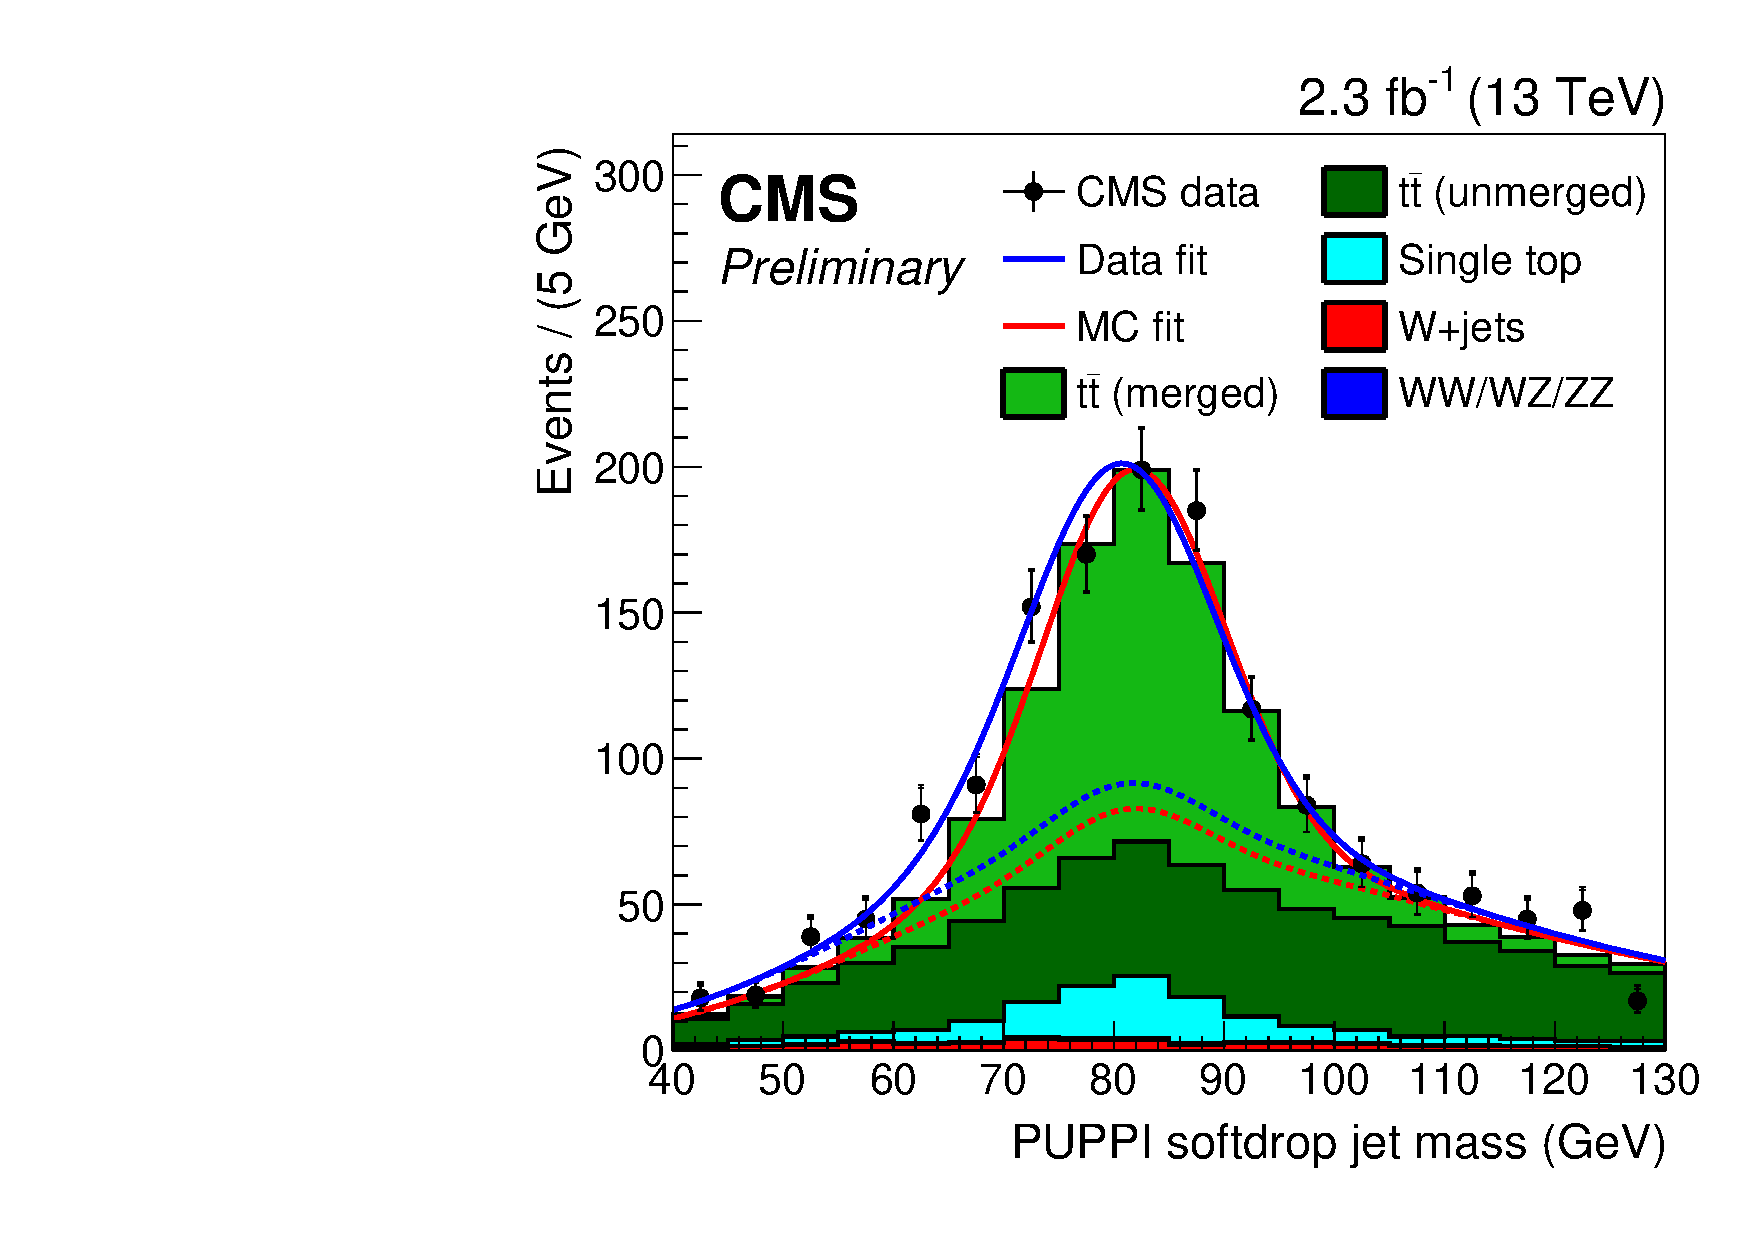
\includegraphics[width=.35\textwidth]{WG3_plots/CMS-PAS-JME-16-003_Figure_018-c}
\hfill
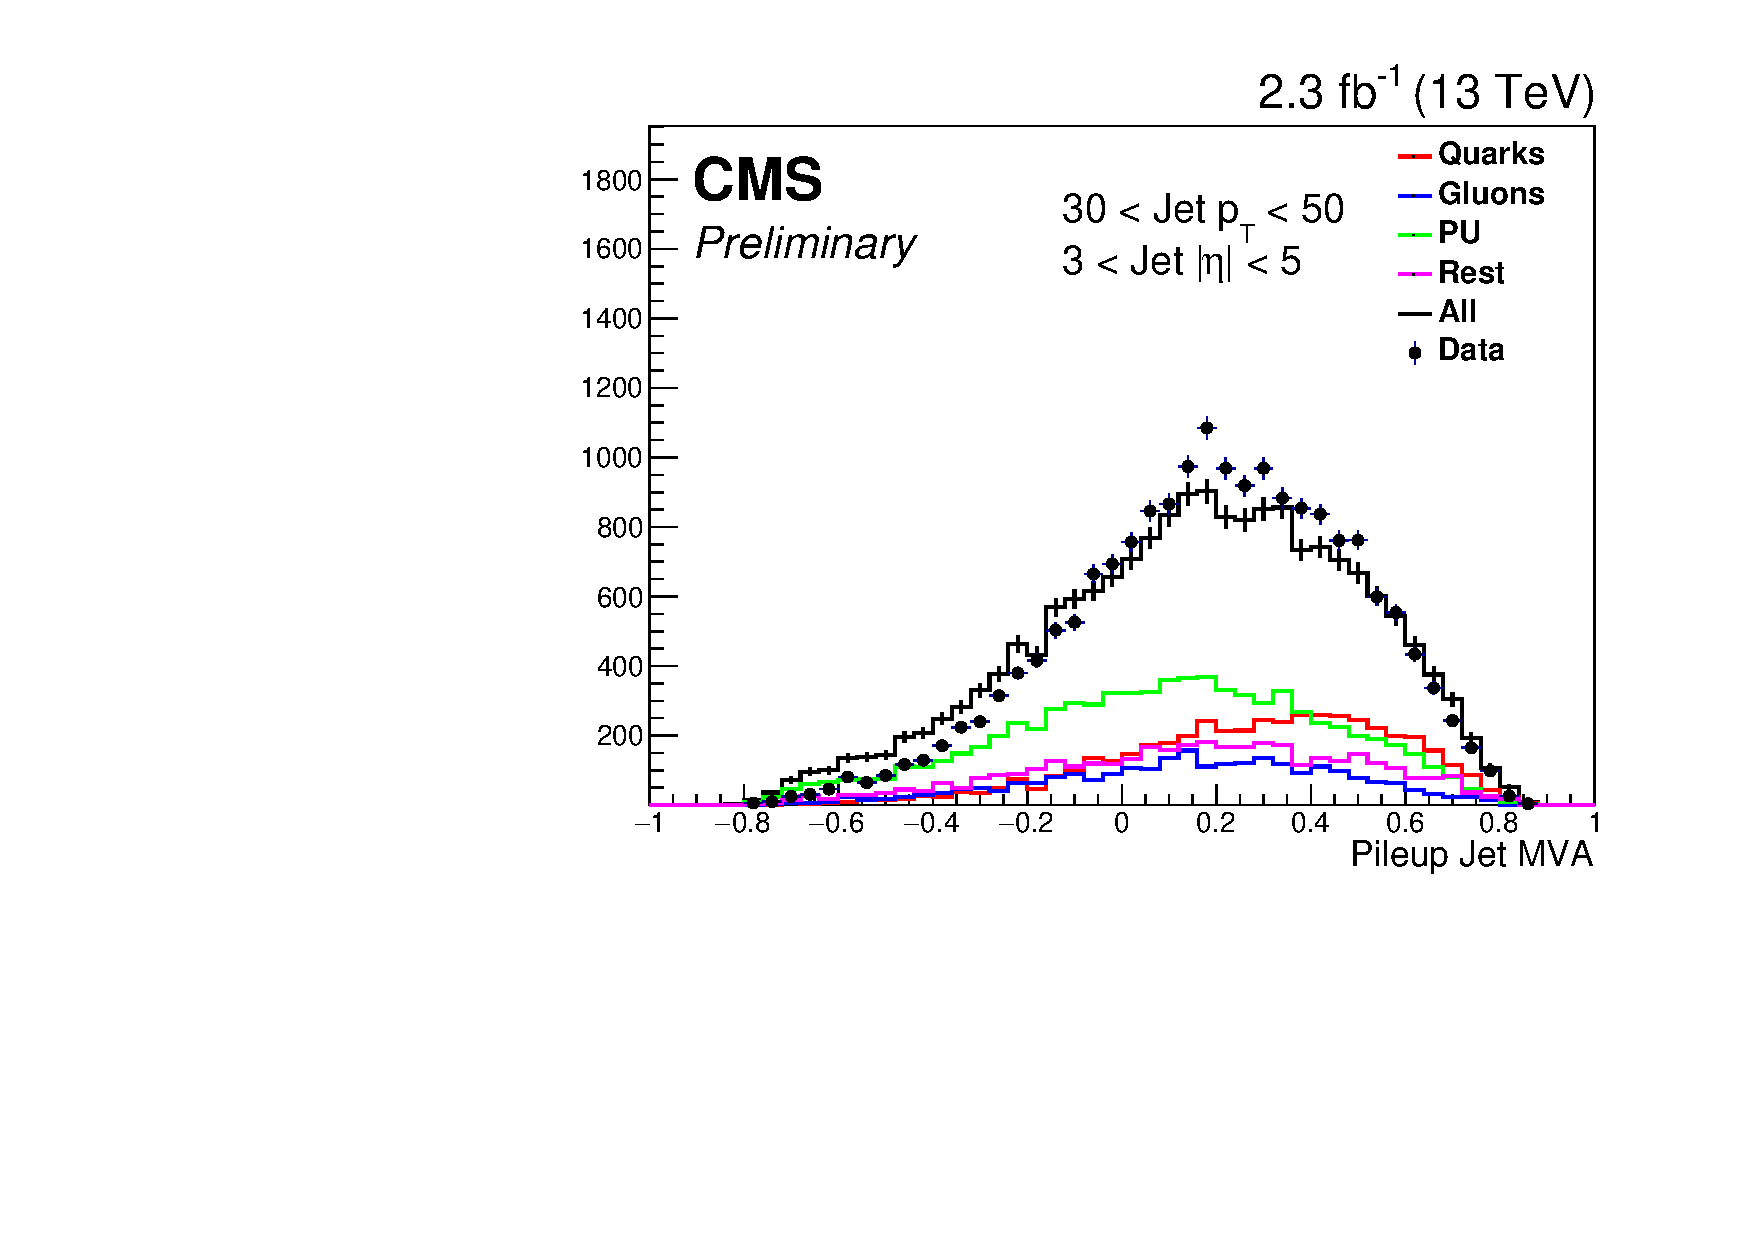
\includegraphics[width=.42\textwidth]{WG3_plots/CMS-PAS-JME-16-003_Figure_014-b}
% \vspace*{-1em}
\caption{(Left) Softdrop jet mass of boosted W bosons in data and simulated samples of top pair production in the single lepton plus jets final state.
(right) Pileup jet MVA discriminator in data and simulation for jets with $|\eta|>3.0$.}
\label{fig:CMSsubstructure}
\end{figure}

Figure~\ref{fig:CMSsubstructure} (left) shows the main observable used by CMS to distinguish W and Z boson jets from quark and gluon initiated jets, the softdrop jet mass, which is the mass of the jet after iteratively removing soft radiation with the modified mass-drop algorithm~\cite{Dasgupta:2013ihk,Butterworth:2008iy}, known as the softdrop algorithm~\cite{Larkoski:2014wba}, a procedure that reduces the mass of quark and gluon jets and improves the mass resolution of W and Z boson jets.
In addition, the substructure of the jet is explored with an N-subjettiness~\cite{Thaler:2010tr} ratio that distinguishes the W and Z boson jets composed of two hard subjets from single quark and gluon jets.
With this combination of observables, a mistag rate of $\sim1$\% at an efficiency of 50\% is achieved for a broad range of transverse momenta from $p_T>200$ GeV up to at least 3.5 TeV.
The jet mass and substructure observables are calibrated using a data sample of top pair production in the single lepton final state containing high-$p_T$ W bosons, achieving uncertainties of the order of 1\% on jet mass scale and 10\% on jet mass resolution and jet substructure tagging efficiency, which increase at higher jet $p_T$ where simulation is used for extrapolation.
Particles from additional interactions happening in the same pp bunch crossing, called pileup interactions, can significantly distort these observables.
CMS thus employs dedicated particle based pileup removal techniques that correct not only jet momenta, but also jet shape or substructure observables.
Charged particles that are identified by the tracking detector to originate from pileup interaction vertices are removed before jet clustering (this procedure is called CHS). For neutral particles a probability weight based on the distribution of surrounding particles following the pileup per particle identification (PUPPI) algorithm~\cite{Bertolini:2014bba} is applied to the particle four momenta~\cite{CMS-PAS-JME-14-001}.
With these pileup suppression techniques, the performance of W and Z boson identification is constant up to at least 40 pileup interactions, and with the higher granularity tracking detector planned for the HL-LHC, performance is maintained up to 200 pileup interactions.
Notable for VBS studies, the longitudinal and transverse polarization of W boson jets can be separated using subjet information, yielding a mistag rate of $\sim$30\% at an efficiency of 50\%.

Also the two forward jets from VBS require an analysis of their substructure, in order to suppress the background from (possibly overlapping) jets originating from pileup interactions~\cite{CMS-PAS-JME-16-003, CMS-PAS-JME-13-005}.
In a scenario of 25 pileup interactions (about half of the pileup expected in Run II of the LHC), without pileup mitigation $\sim$50\% of VBS selected forward jets are from pileup.
Since for $|\eta|>3.0$ no tracking information is available to suppress pileup particles and also jet shape difference are difficult to resolve due to coarse calorimeter granularity ($\Delta \eta \times \Delta \phi = 0.175 \times 0.175$), a multivariate analysis (MVA) is needed to distinguish quark jets from pileup and gluon background.
Figure~\ref{fig:CMSsubstructure} (right) shows the pileup jet MVA discriminator that allows to achieve a pileup mistag rate of $\sim$30\% at a quark efficiency of 50\%.
At the HL-LHC, for which CMS tracking and vertex identification will be extended from $|\eta|<2.5$ to $|\eta|<4$ and a high granularity endcap calorimeter will be installed in the region $1.5<|\eta|<3$, VBS jet identification can rely on the much more powerful CHS and PUPPI pileup rejection techniques.
